\section{Estabilidade de sistemas discretos}

\begin{frame}{Análise da equação característica}
\begin{block}{Função de transferência}
\begin{itemize}
    \item Considere que a função de transferência de um SLIT (sistema linear e invariante no tempo) discreto seja dada como a razão de dois polinômios:
\end{itemize}
	$$H(z) = \dfrac{C(z)}{R(z)} = \dfrac{b_{m}z^{m}+b_{m-1}z^{m-1}+\cdots+b_{1}z+b_{0}}{a_{n}z^{n}+a_{n-1}z^{n-1}+\cdots+a_{1}z+a_{0}}, m < n, a_n \neq 0$$
\end{block}
\end{frame}

\begin{frame}{Análise da equação característica}
\begin{block}{Função de transferência}
\begin{itemize}
    \item Os \textbf{polos} (que determinam a estabilidade de um sistema) são as raízes da \textbf{equação característica}, dada por:
\end{itemize}
$$\boxed{D(z) = a_{n}z^{n}+a_{n-1}z^{n-1}+\cdots+a_{1}z+a_{0}}$$
\end{block}
\vspace{0.4cm}
\centering
\scalebox{0.8}{\deftkzbds
	
\begin{tikzpicture}[auto, node distance=1.5cm,>=Latex]
	
	\node [input, name=input] {};
	\node [sum, right =of input, xshift=0.5cm] (sum) {$ \phantom{\sum} $};
	\draw [draw,->] (input) -- node {$R(z)$} (sum);
	
	\node [block, right =of sum, text width=2cm, align=center] (controller) {$ C(z) $};
	\draw [->] (sum) -- node {$E(z)$} (controller);
	
	\node [block, right =of controller, text width=2cm, align=center] (process) {$ G(z) $};
	\draw [->] (controller) -- node {$U(z)$} (process);
	
	\node [output, right =of process] (output) {};
	\draw [->] (process) -- node [name=y] {$C(z)$}(output);
	
	\node [coordinate,below=of controller, inner sep=0pt] (midp) {};
	\draw[->] (y) |- (midp) -| node[pos=0.98] {$-$} node[pos=1.3] {$+$} (sum);
\end{tikzpicture}}
\end{frame}

\begin{frame}{Análise da equação característica}
\begin{block}{Métodos para verificação da estabilidade}
\begin{itemize}
    \item Para verificar se um dado sistema é \textbf{estável}, a partir de sua equação característica, podemos utilizar os seguintes métodos:
    \begin{enumerate}
        \item Localização dos polos;
        \item Critério de Jury;
        \item Critério de Routh-Hurwitz.
    \end{enumerate}
\end{itemize}
\end{block}
\end{frame}

\begin{frame}{Métodos para verificação da estabilidade}
\begin{block}{Localização dos polos}
\begin{itemize}
    \item \textbf{Condição para estabilidade:}
\end{itemize}
$$\boxed{|p_i| \leq  1, \; i = 1, 2, \cdots, n}$$
\begin{itemize}
    \vspace{-0.3cm}
    \item[] sendo que $p_i$ indica o $i$-ésimo polo de $H(z)$.
    \item Em outras palavras, este método procura determinar se existem polos de $G(z)$ \textbf{fora do círculo de raio unitário}.
    \item Portanto, se pelo menos uma das  raízes de $D(z)$ estiver \textit{fora do círculo de raio unitário}, o sistema é \textbf{instável}.
\end{itemize}
\end{block}
\end{frame}

\begin{frame}{Métodos para verificação da estabilidade}
\begin{block}{Critério de Jury}
\begin{itemize}
    \item Trata-se de uma aplicação direta, utilizando os coeficientes da equação característica.
    \item O teste não diz quantas raízes estão fora do círculo do raio unitário e nem quais são os valores delas (\textit{caso haja}), limitando-se apenas a dizer se o sistema é \textbf{estável} ou \textbf{instável}.
\end{itemize}
\end{block}
\end{frame}

\begin{frame}{Métodos para verificação da estabilidade}
\begin{block}{Critério de Jury}
\begin{itemize}
    \item Deve-se montar um arranjo em forma de uma matriz:
\end{itemize}
$$D(z) = a_{n}z^{n}+a_{n-1}z^{n-1}+\cdots+a_{1}z+a_{0}$$
\vspace{-0.6cm}
\begin{longtable}{cCCCCCC}
	\toprule
	Linha & z^{0} 	& z^{1} & z^{2} & \cdots & z^{n-1} & z^{n}	\\ \midrule
	    1 & a_0		& a_1	& a_2	& \cdots & a_{n-1} & a_n	\\ 
		2 & a_n	& a_{n-1}	& a_{n-2} 	& \cdots	& a_1 & a_0	\\
		3 & b_0		& b_1	& b_2	& \cdots & b_{n-1} & 	\\ 
		4 & b_{n-1}	& b_{n-2}	& b_{n-3} 	& \cdots	& b_0 & \\ 
		5 & c_0		& c_1	& \cdots	& c_{n-2} &  & 	\\ 
		6 & c_{n-2}	& c_{n-3}	& \cdots 	& c_0	&  & \\ 
		\vdots & \vdots & \vdots	& \vdots	&  &  & 	\\ \bottomrule 
\end{longtable}
\vspace{-0.5cm}
$$b_k = \begin{vmatrix}
a_0 & a_{n-k}\\a_n & a_k
\end{vmatrix},
\qquad
c_k = \begin{vmatrix} 
b_0 & b_{n-k-1}\\b_{n-1} & b_k
\end{vmatrix}, \qquad k=0,1,2...$$
\end{block}
\end{frame}

\begin{frame}{Métodos para verificação da estabilidade}
\begin{block}{Critério de Jury}
\begin{itemize}
    \item \textbf{Condições para estabilidade:}
\end{itemize}
\begin{enumerate}
		\item $ D(1)>0 $
		\item $ (-1)^{n}D(-1)>0 $
		\item $ |a_{0}|<|a_{n}| $
		\item $ |b_{0}|>|b_{n-1}| $
		\item $ |c_{0}|>|c_{n-2}| $
\end{enumerate}
	
	\vspace{0.5cm}
	
	\textbf{Atenção!} Deve-se testar $ \boxed{n+1} $ condições! Se \textbf{alguma} condição falhar, então existe pelo menos uma raiz fora do círculo de raio unitário.
\end{block}
\end{frame}

\begin{frame}{Métodos para verificação da estabilidade}
\begin{block}{Critério de Routh-Hurwitz}
\begin{itemize}
    \item Também trata-se de uma aplicação direta, utilizando os coeficientes da equação característica.
    \item Neste caso, deve-se utilizar a \textbf{transformação do plano} \bm{$w$}. Portanto, utiliza-se uma nova equação característica na variável $w$ tal que o número de raízes no \textbf{semiplano direito} é igual ao número de raízes de \textbf{fora do círculo unitário}.
    \item Diferentemente do critério de Jury, este diz quantas raízes estão fora do círculo do raio unitário (\textit{caso haja}). No entanto, também não apresenta quais são os valores destas raízes (\textit{caso haja}).
\end{itemize}
\end{block}
\end{frame}

\begin{frame}{Métodos para verificação da estabilidade}
\begin{block}{Critério de Routh-Hurwitz}
\begin{itemize}
    \item Deve-se montar um arranjo em forma de uma matriz:
\end{itemize}
$$D(w) = a_{n}w^{n}+a_{n-1}w^{n-1}+\cdots+a_{1}w+a_{0}$$
\vspace{-0.6cm}
\begin{longtable}{CCCC}
	\toprule
		a_n	& a_{n-2} & a_{n-4} & \cdots	 \\
		a_{n-1}	& a_{n-3} & a_{n-5}	& \cdots \\ 
		b_1 & b_2 & b_3 & \cdots \\ 
		c_1 & c_2 & c_3 & \cdots \\
		\vdots & \vdots & \vdots & \ddots \\ \bottomrule 
\end{longtable}
$$b_i = \dfrac{a_{n-1} \cdot a_{n-2i} - a_n \cdot a_{n-(2i+1)}}{a_{n-1}}$$
$$c_i = \dfrac{b_1 \cdot a_{n-(2i+1)} - a_{n-1} \cdot b_{i+1}}{b_1}$$
\end{block}
\end{frame}

\begin{frame}{Exemplo \#01}
\begin{block}{Problema}
	\[ D(z)=z^{3}-\num{1,25}z^{2}-\num{1,3}z-\num{0,25} \]
\end{block}
\end{frame}

\begin{frame}{Exemplo \#01}
\begin{block}{Resolução - localização dos polos}
\begin{itemize}
    \item Utilizando um software computacional como, por exemplo, o \MATLAB, temos que os três polos estão localizados em:
\end{itemize}
$$z_1 = \num{1,97}$$
$$z_2 = -\num{0,42}$$
$$z_3 = -\num{0,30}$$
\begin{itemize}
    \item Como $|z_1| = \num{1,97} > 1$, o sistema é \textbf{instável}.
\end{itemize}
\end{block}
\end{frame}

\begin{frame}{Exemplo \#01}
\begin{block}{Resolução - critério de Jury}
\begin{itemize}
	\item Comparando com 
	$$D(z) = a_{n}z^{n}+a_{n-1}z^{n-1}+\cdots+a_{1}z+a_{0},$$
\end{itemize}
\begin{itemize}
    \item[] temos que $n=3$, logo \textbf{deve-se testar 4 condições.}
\end{itemize}
\begin{enumerate}[(1)]
	\item $D(1)>0 \implies 1^{3}-\num{1,25}\cdot1^{2}-\num{1,3}\cdot1-\num{0,25}=-\num{1,8}>0 \quad \text{\xmark}$
\end{enumerate}
\begin{itemize}
    \item Como a primeira condição não foi satisfeita, o sistema é \textbf{instável}.
\end{itemize}
\end{block}
\end{frame}

\begin{frame}{Exemplo \#01}
\begin{block}{Resolução - critério de Routh-Hurwitz}
\begin{itemize}
	\item Considerando o caso particular da transformação entre os planos $z$ e $w$ (\textit{onde o tempo de amostragem não é considerado}), temos que
\end{itemize}
$$z = \dfrac{w+1}{w-1}$$
\begin{itemize}
    \item Substituindo em $D(z)=z^{3}-\num{1,25}z^{2}-\num{1,3}z-\num{0,25}$, e igualando a zero:
\end{itemize}
$$\left(\dfrac{w+1}{w-1}\right)^3 - \num{1,25}\left(\dfrac{w+1}{w-1}\right)^2 - \num{1,3}\left(\dfrac{w+1}{w-1}\right) - \num{0,25} = 0$$
\begin{itemize}
    \item Após manipulações algébricas, temos:
\end{itemize}
$$-\num{1,8}w^{3}+\num{3,8}w^{2}+\num{4,8}w+\num{1,2} = 0$$
\end{block}
\end{frame}

\begin{frame}{Exemplo \#01}
\begin{block}{Resolução - critério de Routh-Hurwitz}
\begin{itemize}
    \item O arranjo fica, portanto:
\end{itemize}
\begin{longtable}{CC}
	\toprule
		-\num{1,8} & \num{4,8}	 \\
		 \num{3,8} & \num{1,2}	 \\
		 \num{5,4} &         	 \\
		 \num{1,2} &        	 \\
	\bottomrule 
\end{longtable}
\begin{itemize}
    \item Como houve uma mudança de sinal na primeira coluna, sabemos que existe um polo fora do círculo unitário. Sendo assim, o sistema é \textbf{instável}.
\end{itemize}
\end{block}
\end{frame}

\begin{frame}{Exemplo \#02}
\begin{block}{Problema}
	\[ D(z)=z^{3}+\num{2,1}z^{2}+\num{2,08}z+\num{0,64} \]
\end{block}
\end{frame}

\begin{frame}{Exemplo \#02}
\begin{block}{Resolução - localização dos polos}
\begin{itemize}
    \item Utilizando um software computacional como, por exemplo, o \MATLAB, temos que os três polos estão localizados em:
\end{itemize}
$$z_1 = -\num{0,8} + j\num{0,8}$$
$$z_1 = -\num{0,8} - j\num{0,8}$$
$$z_3 = -\num{0,5}$$
\begin{itemize}
    \item Como $|z_1| = |z_2| = \num{1,13} > 1$, o sistema é \textbf{instável}.
\end{itemize}
\end{block}
\end{frame}

\begin{frame}{Exemplo \#02}
\begin{block}{Resolução - critério de Jury}
\begin{itemize}
	\item Comparando com 
	$$D(z) = a_{n}z^{n}+a_{n-1}z^{n-1}+\cdots+a_{1}z+a_{0},$$
\end{itemize}
\begin{itemize}
    \item[] temos que $n=3$, logo \textbf{deve-se testar 4 condições.}
\end{itemize}
\begin{enumerate}[(1)]
	\item $D(1)>0 \implies 1^{3}+\num{2,1}\cdot1^{2}+\num{2,08}\cdot1+\num{0,64}=\num{5,82}>0 \quad \text{\cmark}$
	\item $(-1)^{n}D(-1)>0 \implies -1\left[ (-1)^{3}+\num{2,1}(-1)^{2}+\num{2,08}(-1)+\num{0,64} \right]=\num{0,34}>0 \quad \text{\cmark}$
	\item $|a_{0}|<|a_{3}| \implies \num{0,64} < 1 \quad \text{\cmark}$
\end{enumerate}
\end{block}
\end{frame}

\begin{frame}{Exemplo \#02}
\begin{block}{Resolução - critério de Jury}
\begin{enumerate}
	\item[(4)] $|b_{0}|>|b_{2}|$
\end{enumerate}
\vspace{-0.5cm}
\begin{longtable}{cCCCC}
	\toprule
	Linha & z^{0} 	& z^{1} & z^{2} & z^{3}	\\ \midrule
		1 & \num{0,64}	& \num{2,08}	& \num{2,1} 	& 1		\\
		2 & 1 		& \num{2,1}	& \num{2,08}	& \num{0,64}	\\ \bottomrule
\end{longtable}

\vspace{-0.3cm}

\[ \left. \begin{aligned}
b_{0}&=\begin{vmatrix}
\num{0,64} & 1\\1 & \num{0,64}
\end{vmatrix}=\num{-0,5904}\\
b_{1}&=\begin{vmatrix}
\num{0,64} & \num{2,1}\\1 & \num{2,08}
\end{vmatrix}=-\num{0,7688}\\
b_{2}&=\begin{vmatrix}
\num{0,64} & \num{2,08}\\1 & \num{2,1}
\end{vmatrix}=-\num{0,7360}
\end{aligned}\right\rbrace |b_{0}|>|b_{2}| \implies \num{0,5904} > \num{0,7360} \quad \text{\xmark} \]
\vspace{-0.2cm}
\begin{itemize}
    \item Como a quarta condição não foi satisfeita, o sistema é \textbf{instável}.
\end{itemize}
\end{block}
\end{frame}

\begin{frame}{Exemplo \#02}
\begin{block}{Resolução - critério de Routh-Hurwitz}
\begin{itemize}
	\item Considerando o caso particular da transformação entre os planos $z$ e $w$ (\textit{onde o tempo de amostragem não é considerado}), temos que
\end{itemize}
$$z = \dfrac{w+1}{w-1}$$
\begin{itemize}
    \item Substituindo em $D(z)=z^{3}+\num{2,1}z^{2}+\num{2,08}z+\num{0,64}$, e igualando a zero:
\end{itemize}
$$\left(\dfrac{w+1}{w-1}\right)^3 + \num{2,1}\left(\dfrac{w+1}{w-1}\right)^2 + \num{2,08}\left(\dfrac{w+1}{w-1}\right) + \num{0,64} = 0$$
\begin{itemize}
    \item Após manipulações algébricas, temos:
\end{itemize}
$$\num{5,82}w^{3}+\num{1,1}w^{2}+\num{0,74}w+\num{0,34} = 0$$
\end{block}
\end{frame}

\begin{frame}{Exemplo \#02}
\begin{block}{Resolução - critério de Routh-Hurwitz}
\begin{itemize}
    \item O arranjo fica, portanto:
\end{itemize}
\begin{longtable}{CC}
	\toprule
		  \num{5,82} & \num{0,74} \\
		  \num{1,1}  & \num{0,34} \\
		 -\num{1,05} &         	  \\
		  \num{0,34} &        	  \\
	\bottomrule 
\end{longtable}
\begin{itemize}
    \item Como houve duas mudanças de sinal na primeira coluna, sabemos que existem dois polos fora do círculo unitário. Sendo assim, o sistema é \textbf{instável}.
\end{itemize}
\end{block}
\end{frame}












\begin{frame}{Exemplo \#03}
\begin{block}{Problema}
Dado o sistema representado na figura abaixo, e considerando um controlador proporcional, ou seja, $ C(z)=K $, encontre o range de valores de $ K $ para que o sistema em malha fechada seja estável.

\[ G(z)=\dfrac{z-1}{(z-\num{0,1})(z-\num{0,8})} \]
\end{block}

\vspace{0.5cm}

\centering

\scalebox{0.7}{\deftkzbds
	
\begin{tikzpicture}[auto, node distance=1.5cm,>=Latex]
	
	\node [input, name=input] {};
	\node [sum, right =of input, xshift=0.5cm] (sum) {$ \phantom{\sum} $};
	\draw [draw,->] (input) -- node {INPUT} (sum);
	
	\node [block, right =of sum, text width=2cm, align=center] (controller) {$ C(z) $};
	\draw [->] (sum) -- (controller);
	
	\node [block, right =of controller, text width=2cm, align=center] (process) {$ G(z) $};
	\draw [->] (controller) -- (process);
	
	\node [output, xshift=1cm, right =of process] (output) {};
	\draw [->] (process) -- node [name=y] {OUTPUT}(output);
	
	\node [coordinate,below=of process, inner sep=0pt] (midp) {};
	\draw[->] (y) |- (midp) -| node[pos=0.98] {$-$} node[pos=1.3] {$+$} (sum);
\end{tikzpicture}}
\end{frame}


\begin{frame}{Exemplo \#03}
\begin{block}{Resolução}
	\[ H(z)=\dfrac{C(z)G(z)}{1+C(z)G(z)}=\frac{K(z-1)}{(z-\num{0,1})(z-\num{0,8})+K(z-1)}\]
	
	Equação característica: $ (z-\num{0,1})(z-\num{0,8})+K(z-1)=0 \,\Rightarrow\, z^{2}+(K-\num{0,9})z+\num{0,08}-K=0 $
	
	\begin{enumerate}[(1)]
		\item $ D(1)>0 \implies 1\cancel{+K}-\num{0,9}+\num{0,08}\cancel{-K}>0=\num{0,18}>0\quad\text{\cmark} $
		\item $ (-1)^{n}D(-1)>0 \implies (-1)^{2}+(K-\num{0,9})(-1)+\num{0,08}-K>0\,\Rightarrow\, -2K>-1,98\,\Rightarrow\, K<\num{0,99} $
		\item $ |a_{0}|<|a_{3}| \implies |\num{0,08}-K| < 1 \, \rightarrow\, \num{0,92}>-K \, \Rightarrow\, K>-\num{0,92} $
	\end{enumerate}

	\[ \text{Logo, }-\num{0,92}<K<\num{0,99} \]
\end{block}
\end{frame}


\frame{
\frametitle{Exercícios}
\begin{block}{}
01. Avalie a estabilidade (utilizando os seguintes métodos:  i - localização dos polos; ii - critério de Jury; iii - critério de Routh-Hurwitz) correspondentes às seguintes equações características: 
    \vspace{0.3cm}
\begin{enumerate}
    \item[(a)]$D(z)=z^3+\num{3,5}z^2+4z+\num{0,8}$
    \vspace{0.3cm}
    \item[(b)]$D(z)=z^2-z+2$
\end{enumerate}

\vspace{0.7cm}

02. Considere a equação característica de um sistema como sendo:
$$1 + \dfrac{Kz(1 - \text{e}^{-T})}{(z-1)(z-\text{e}^{-T})} = 0$$
Aplique o critério de estabilidade de Jury para determinar a faixa de valores do tempo de amostragem $T$ para o qual o sistema é estável, para um dado valor de $K$.
\end{block}
}

\frame{
\frametitle{Exercícios}
\begin{block}{}
03. Considere um sistema dinâmico descrito pela equação de diferenças:
$$y[k+2]-y[k+1]+ \alpha y[k] = u[k]$$
Dado que $G(z)=Y(z)/U(z)$, determine para quais valores de $\alpha$ o sistema $G(z)$ é estável.

\vspace{0.7cm}

04. Utilize o critério de Jury para determinar a faixa de valores de $K$ tais que o sistema em  malha fechada ilustrado na figura abaixo seja estável. Confirme o resultado por meio do critério de Routh-Hurwitz.
\end{block}
\centerline{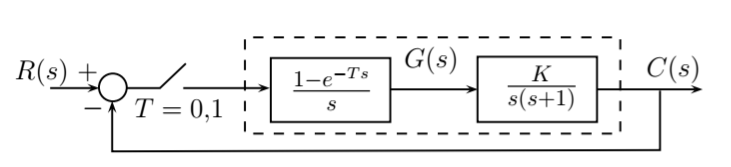
\includegraphics[width=0.9\linewidth]{Figuras/Ch07/fig1.PNG}}
}

\frame{
\frametitle{Referências e exercícios complementares}
\begin{itemize}
\item AGUIRRE, Luis A. Controle de Sistemas Amostrados, 1 ed. [s.n.], 2019.
\end{itemize}
\centering{\alert{Página 179 - \textbf{Capítulo 5}}} \\
\vspace{0.4cm}
\begin{itemize}
\item FRANKLIN, Gene F.; POWELL, J. David; WOLKMAN, Michael L. Digital Control of Dynamic Systems, 3 ed. Addison-Wesley, 1998.
\end{itemize}
\centering{\alert{Página 149 - \textbf{Capítulo 4}}} \\
}